\documentclass[border=10pt]{standalone}

\usepackage{tikz}
\usepackage{tikzsymbols}
\usetikzlibrary{calc,patterns,shapes.geometric}

\def\centerarc[#1](#2)(#3:#4:#5){\draw[#1] ($(#2)+({#5*cos(#3)},{#5*sin(#3)})$) arc (#3:#4:#5);}

\begin{document}
	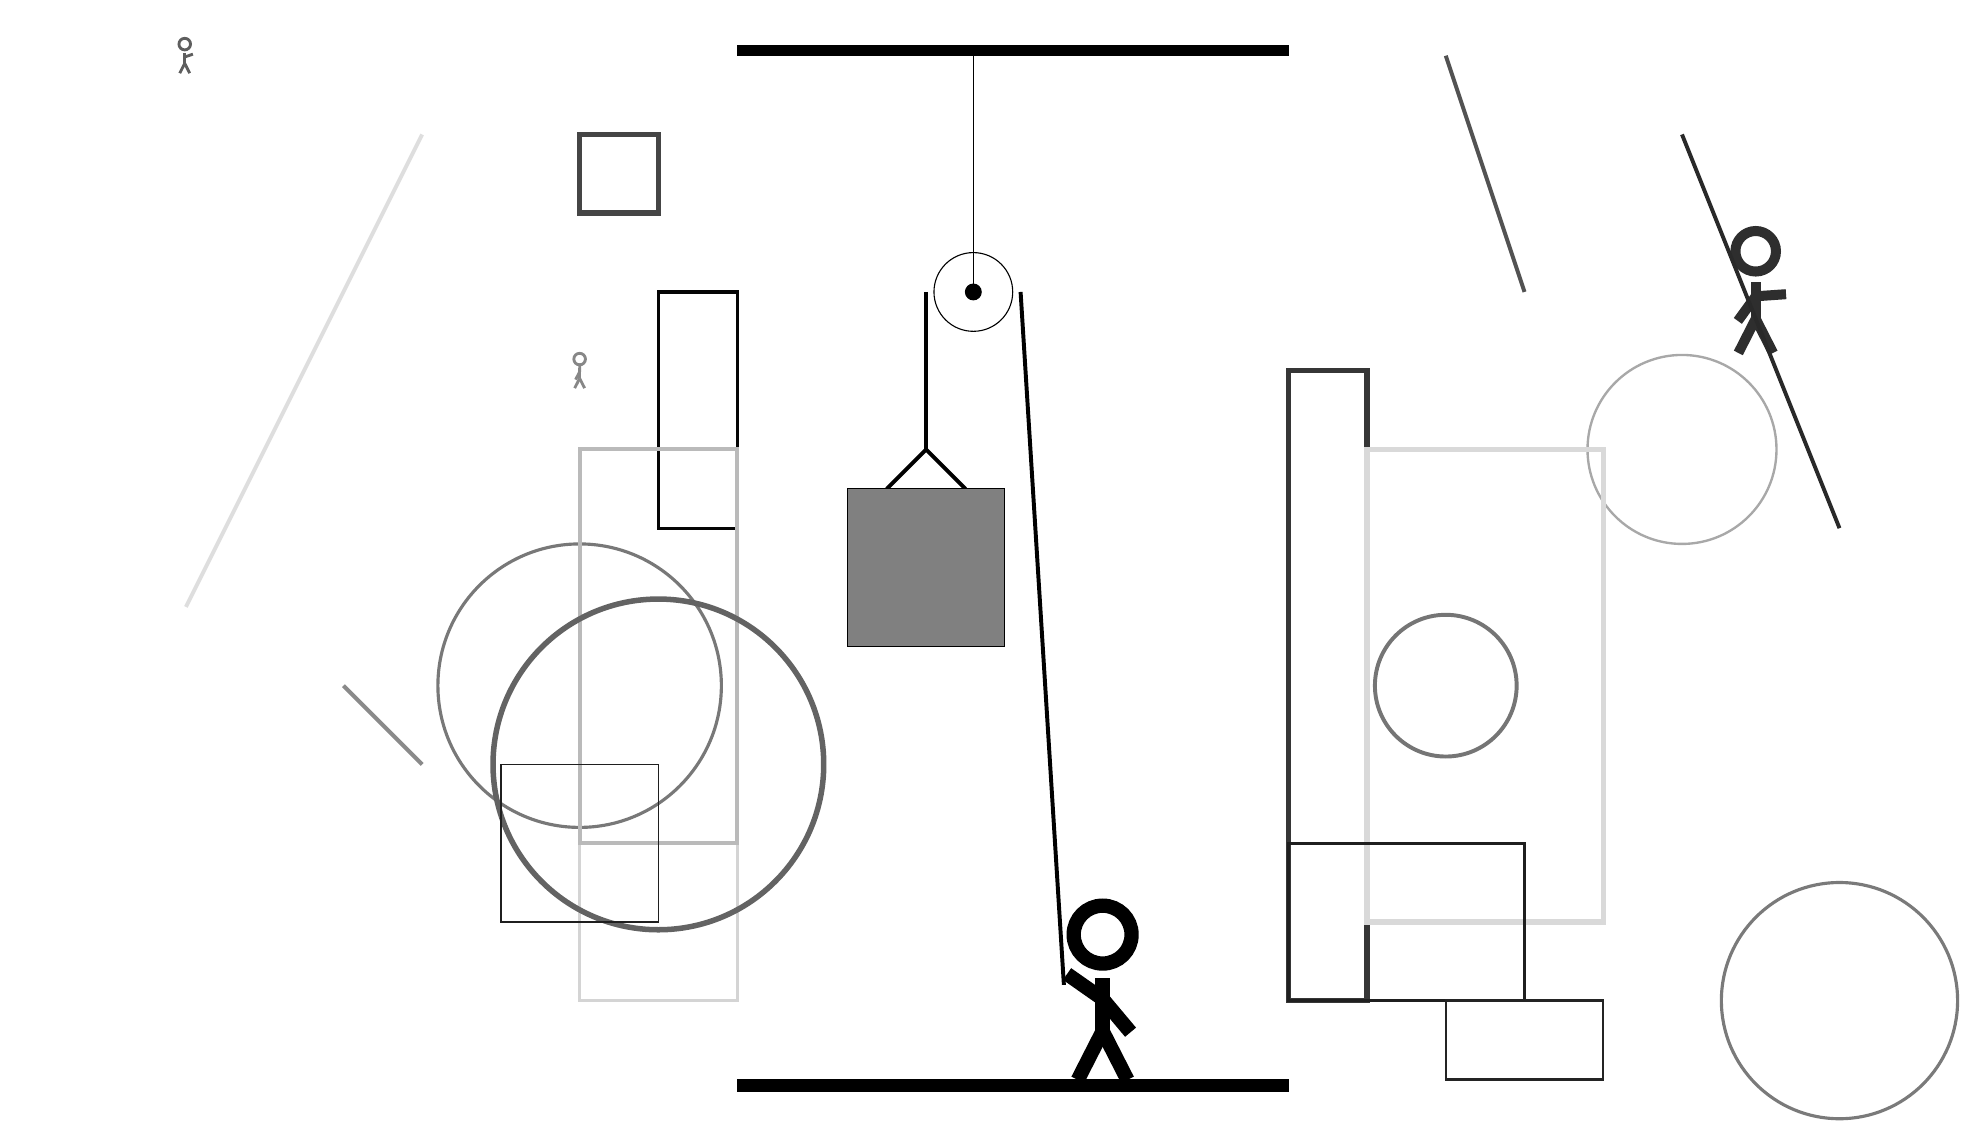
\begin{tikzpicture}
		%%%%% START %%%%%
		
		\draw[fill=black] (-2, 10) rectangle (5, 10.125);
		
		\draw (1, 7) circle (0.5);
		\draw[fill=black] (1, 7) circle (0.1);
		\draw (1, 10) -- (1, 7);
		
		\draw [line width=0.4mm, color=black!52](12, -2) circle (1.5);
		
		\draw [line width=0.3mm, color=black!34](10, 5) circle (1.2);
		\draw[line width=0.4mm, color=black!17] (-2, -2) rectangle (-4, 0);
		\draw[line width=0.5mm, color=black!46](-7, 2) -- (-6, 1);
		\draw [line width=0.4mm, color=black!53](-4, 2) circle (1.8);
		
		\draw[line width=0.7mm, color=black!73] (-4, 8) rectangle (-3, 9);
		
		\node[line width=0.3mm, color=black!82] at (11, 7) {\Strichmaxerl[7][54][4]};
		\draw[line width=0.7mm, color=black!79] (6, 6) rectangle (5, -2);
		\draw[line width=0.7mm, color=black!15] (6, -1) rectangle (9, 5);
		
		\node[line width=0.3mm, color=black!63] at (-9, 10) {\Strichmaxerl[2][90][19]};
		
		\draw [line width=0.5mm, color=black!54](7, 2) circle (0.9);
		\draw[line width=0.5mm, color=black!13](-6, 9) -- (-9, 3);
		\node[line width=0.3mm, color=black!47] at (-4, 6) {\Strichmaxerl[2][62][89]};
		
		\draw[line width=0.4mm, color=black!98] (-3, 4) rectangle (-2, 7);
		\draw [line width=0.2mm, color=black!95](-11, 6) circle (0.0);
		\draw[line width=0.5mm, color=black!84](10, 9) -- (12, 4);
		
		\draw[line width=0.5mm, color=black!27] (-2, 5) rectangle (-4, 0);
		\draw[line width=0.5mm, color=black!68](8, 7) -- (7, 10);
		\draw [line width=0.7mm, color=black!61](-3, 1) circle (2.1);
		
		\draw[line width=0.2mm, color=black!88] (-3, -1) rectangle (-5, 1);
		\draw[line width=0.4mm, color=black!88] (5, 0) rectangle (8, -2);
		
		\draw[line width=0.3mm, color=black!86] (7, -3) rectangle (9, -2);
		
		
		\draw[line width=0.5mm] (-0.1, 4.5) -- (0.4, 5.0) -- (0.9, 4.5);
		\draw[fill=black!50] (-0.6, 4.5) rectangle (1.4, 2.5);
		
		\draw[line width=0.5mm] (0.4, 7) -- (0.4, 5.0);
		\centerarc[line width=0.5mm](1, 7)(0:180:0.6);
		\draw[line width=0.5mm](1.6, 7) -- (2.15, -1.8);
		
		\node at (2.6, -1.9) {\Strichmaxerl[10][-35][-50]};
		
		\draw[fill=black] (-2, -3) rectangle (5, -3.15);
		
		%%%%% END %%%%%
	\end{tikzpicture}
\end{document}